\documentclass[a4paper]{article}
\usepackage[T1]{fontenc}
\usepackage[utf8]{inputenc}
\usepackage[margin=1in]{geometry}
\usepackage[english]{babel}
\usepackage{charter}
\usepackage{graphicx}
\usepackage{parskip}
\usepackage{mathtools}
\usepackage{amssymb}
\usepackage{xfrac}
\usepackage{booktabs}
\usepackage{longtable}
\usepackage{hyperref}


\usepackage{setspace} % increase interline spacing slightly
\setstretch{1}

\def\arraystretch{1} % increase tabular cells padding

\title{
\Large{Big Data Analytics 2019}\\
\huge{NY City Taxi Data Analysis}\\
\large{Project}}

\author{
Prof. Marcel Graf\\
Prof. Nastaran Fatemi\\
\\
Romain Claret, Jämes Ménétrey and Damien Rochat\\
MSE Master of Science in Engineering\\
HES-SO University of Applied Sciences and Arts
\date{\today}}

\begin{document}
\maketitle

\tableofcontents
\clearpage

\section{Introduction}
The goal of this project is to identify the busiest areas from New York City, from a taxi agency perspective, in order to open new agency locations, to increase profit, the taxi availability and more globally the customers' satisfaction. This analysis aims to highlight two topics of interest:

\begin{itemize}
    \item Find the best spots to find customers
    \item Identify the most profitable spots (proportional to the longest trips)
\end{itemize}

To help the authors to achieve those objectives and to handle the big data related dataset, they will be using Spark and more specifically PySpark (the Python implementation of Apache Spark), to process the data and perform machine learning.


\section{Dataset}
The dataset, provided by Chris Whong \footnote{\url{http://www.andresmh.com/nyctaxitrips/}}, is the list of trips and fares for taxis in New York City, for the year 2013. It is composed of 2 parts, which are themselves fragmented into 12 CSV files, one per month, and for a total of 173'179'759 records.

\begin{itemize}
    \item The trips related information (trip\_data.7z, sized 4.1GB)
    \begin{itemize}
        \item Taxi identification
        \item Driver identification
        \item Start time and end time
        \item GPS coordinates of pick up and drop off
    \end{itemize}
    \item The fares related information to each trip (trip\_fare.7z, sized 1.72GB)
    \begin{itemize}
        \item Taxi identification
        \item Driver identification
        \item Start time and end time
        \item Fare information (amount, payment type, tip)
    \end{itemize}
\end{itemize}

\textbf{trip\_data.printSchema()}
\begin{verbatim}
root
 |-- vendor_id: string (nullable = true)
 |-- rate_code: string (nullable = true)
 |-- store_and_fwd_flag: string (nullable = true)
 |-- pickup_datetime: string (nullable = true)
 |-- dropoff_datetime: string (nullable = true)
 |-- passenger_count: string (nullable = true)
 |-- trip_time_in_secs: string (nullable = true)
 |-- trip_distance: string (nullable = true)
 |-- pickup_longitude: string (nullable = true)
 |-- pickup_latitude: string (nullable = true)
 |-- dropoff_longitude: string (nullable = true)
 |-- dropoff_latitude: string (nullable = true)
 \end{verbatim}
 

\textbf{trip\_fare.printSchema()}
\begin{verbatim}
 root
 |-- medallion: string (nullable = true)
 |-- hack_license: string (nullable = true)
 |-- vendor_id: string (nullable = true)
 |-- pickup_datetime: timestamp (nullable = true)
 |-- payment_type: string (nullable = true)
 |-- fare_amount: double (nullable = true)
 |-- surcharge: double (nullable = true)
 |-- mta_tax: double (nullable = true)
 |-- tip_amount: double (nullable = true)
 |-- tolls_amount: double (nullable = true)
 |-- total_amount: double (nullable = true)
 \end{verbatim}

\section{Preprocessing}
This section covers the manipulations performed to clean up the data in order to make it eligible to be processed by the machine learning algorithms.

\subsection{Out of bound GPS coordinates}
After visualizing the GPS coordinates on an interactive map, several of the trips were out of the bounds of New York City. They represented about 1.75\% of the trips. As those trips were not related to our objectives, the trips initiated out of NYC were drop in order to keep the clusters' centroids within the city.

\subsection{Invalid fares}
Some of the trip fares were considered invalid; indeed, their values were either null or equal to zero. They represented about 1\% of the records. The fares are used for the second objective, which determines the most profitable spots to set up taxi agencies or pickup spots. Therefore, those records were curated for the second objective.

\section{Machine learning}
The project relied heavily on machine learning for the two objectives. As the first objective is to determine the best locations for building taxi agencies, a good approach is to create customers clusters per region. The centroid of these clusters inherently become the taxi best spots; those clusters are calculated via the K-Means algorithm. The number of clusters required can be hyper-parametered via the value of $k$. The number of clusters depends on how many agencies the taxi company is willing to open. For that purpose, an interval of values have been selected, so the company can review the results and decide their expansion strategy based on what makes more sense.

The second objective is similar to the first one, but it weights the location of the customers with the fares they have paid for the trip.



\subsection{Features selection}
The GPS coordinates represent the fundamental data that are used to determine the centroids of the clusters. Indeed, this project exploits the fact that the means of the GPS locations are meaningful, as they represent coordinates as well and can be plotted on a map. The data set is comprised of multiple fares values and it has been decided to sum the \emph{fare amount} and the \emph{surchage}, which correspond to an additional amount for night trips. An analysis has been performed on the distribution of the sum of fares, in order to alleviate any outliners that can harm the results. Figure \ref{fig:distribution-fares-bad} illustrates the distribution of the fares over the trips. It appears clears there is a gaussian distribution at the left of the chart and several heavy outliners distort the result. For that purpose, the maximum amount of fares has been set to 20\$, as it keeps the original form of the gaussian, as shown on Figure \ref{fig:distribution-fares-fixed}.

%TODO
max fare value is \$ WTF?? 

\begin{figure}
  \centering
  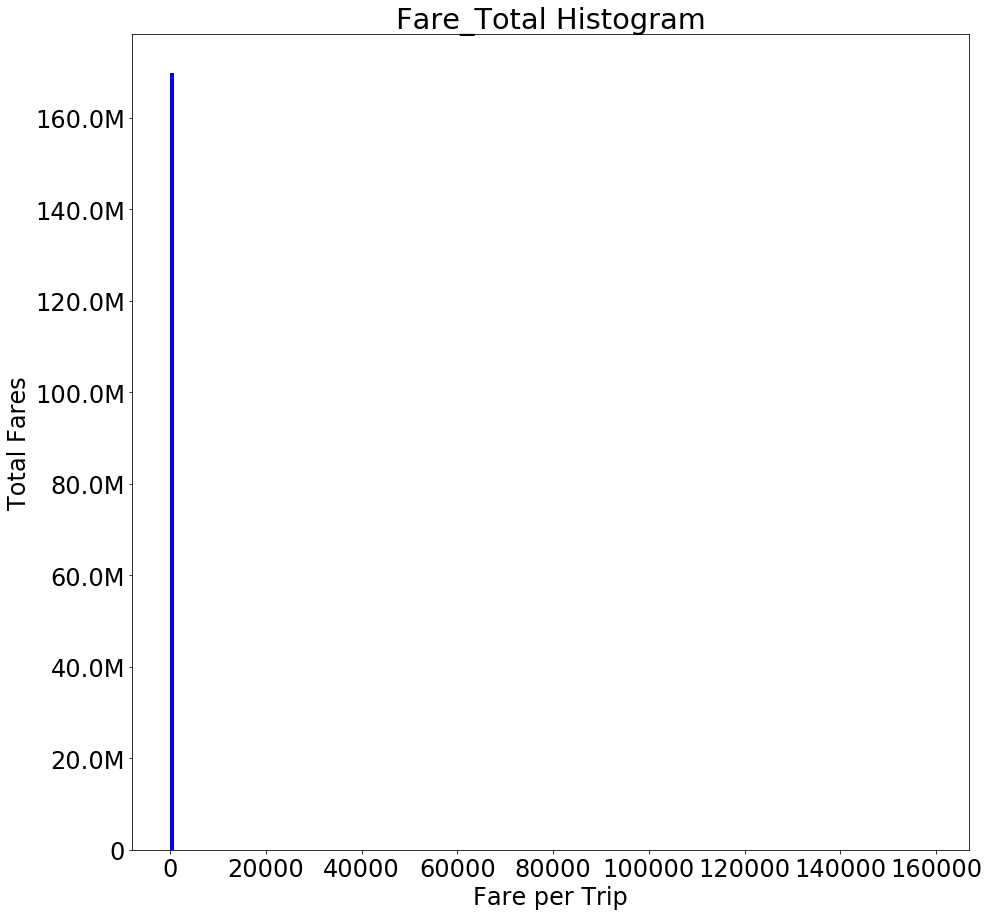
\includegraphics[width=0.6\textwidth]{images/distribution-fares-bad.png}
  \caption{The distribution of the fares over the number of trips.}
  \label{fig:distribution-fares-bad}
\end{figure}

\begin{figure}
  \centering
  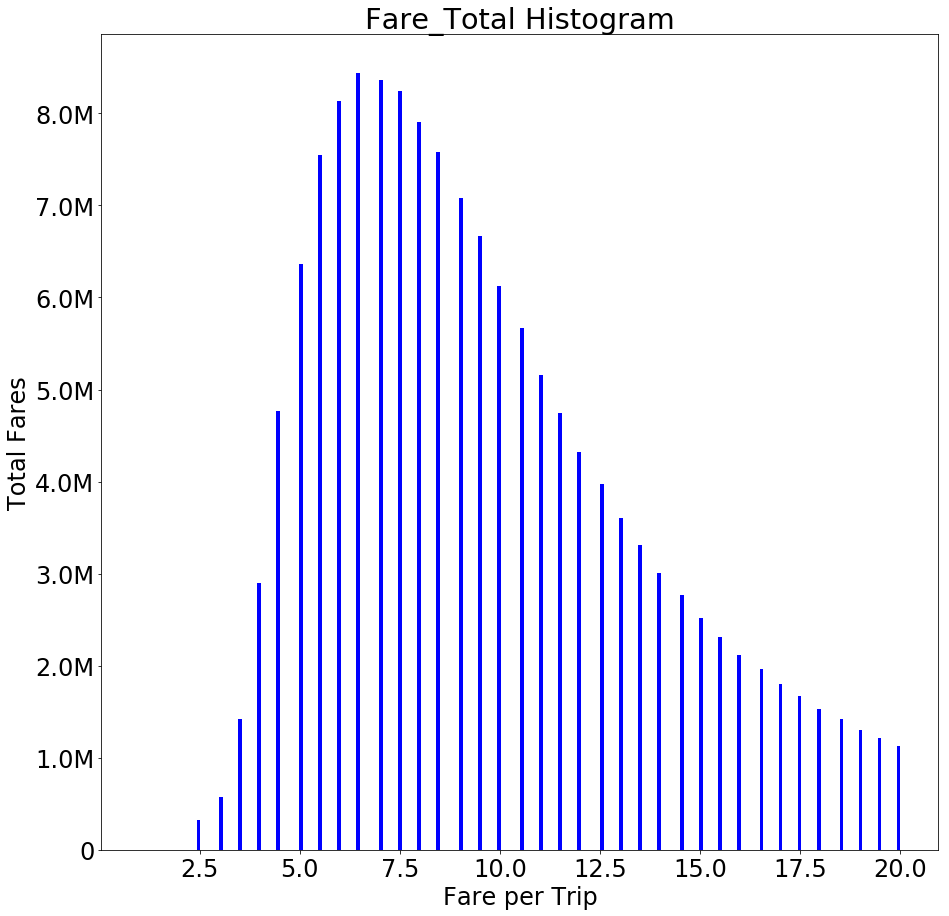
\includegraphics[width=0.6\textwidth]{images/distribution-fares-fix.png}
  \caption{The distribution of the fares adapted for the machine learning.}
  \label{fig:distribution-fares-fixed}
\end{figure}


\subsection{Algorithms}
The K-means algorithm has been used to accomplish the two objectives of the project. The hyperparameters are detailed in the list below:

% TODO Hyperparameters
\begin{itemize}
  \item $X=Y$, because ...
  \item blaa
\end{itemize}


\subsection{Optimizations}
\subsubsection{Sampling the fares}
The computation of the centroids of the second objective have been optimized to take into account the fares of the trips. Indeed, the algorithm of K-means implemented in spark does not provide a way to weight the records differently, based on a value, which would be the flare in the case of the project. The intuitive solution to solve introduction the notion of weight has been to duplicate each record proportionally of its amount of fare. Thanks to this process, a given record has a stronger attraction with the centroids. Obviously, creating new records of amount equal to the fares complexify drastically the initial model, as it increased its size of data set of 2'575\%. That size is so large that it took days to compute a single K-means.

The sampling of the fares has been introduced to circumvent that issue. In a similar process of the sampling of music by famous compression algorithms such as MP3, the fares have been grouped by adjacent values and the index of the group has been used instead of the value of the amount, in order to weight in a lighter way the records. Figure \ref{fig:distribution-fares-sampled} illustrates that the fares have been sampled using three groups. The index of the groups are then used to determine how much time the record must be duplicated, in order to generate to have a stronger gravity.

\begin{figure}
  \centering
  %\includegraphics[]{images/distribution-fares-sampled-png}
  \caption{The sampled distribution of fares.}
  \label{fig:distribution-fares-sampled}
\end{figure}


\section{Testing and evaluation}

\section{Results}
% Web app

\section{Conclusion}
\subsection{Next steps}

\end{document}
























